\chapter{Marco Teórico}

\section{Contexto general del proyecto}

\begin{figure}[h]
\centering
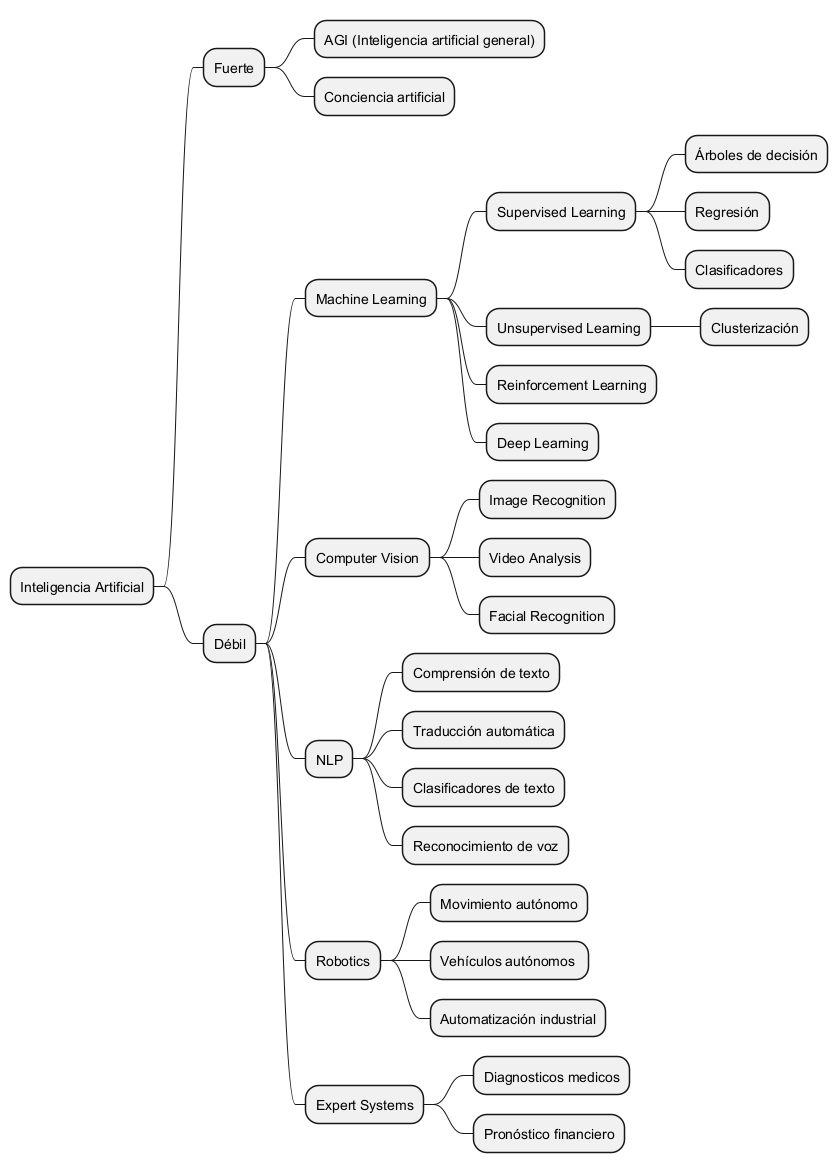
\includegraphics[width=0.5\textwidth]{imagenes/marcoTeorico/DiagramaRamasAI.png}
\caption{Diagrama de IA}
\label{fig:iadiagram}
\end{figure}

El presente proyecto se fundamenta en la rama del aprendizaje de maquina, puntualmente en el aprendizaje profundo en lo que se refiere a los modelos largos del lenguaje.
Los conocidos como LLMs son estructuras que contemplan redes neuronales profundas y múltiples capas, Estas redes neuronales pueden procesar textos e intrucciones al nivel del lenguaje humano lo que les permite desempeñar diferentes tareas relacionadas con texto principalmente, como lo pueden ser las tareas de generación de texto y las tareas de clasificación siendo estas últimas el tipo principal de tarea con la que se trabajara a lo largo del presente proyecto.

\subsection{Que son los modelos largos de lenguaje LLM y cual es su utilidad}
%2025/08/27  papper de attention is all u need: revisar si es requerido para incluir en marco teorico https://arxiv.org/abs/1706.03762

% FUENTES POSIBLES DE CONSULTA (NO INCLUIDAS AUN)
%https://developers.google.com/s/results/machine-learning?hl=es-419&q=llms%20foundations


Los modelos largos de lenguajes o modelos de lenguaje de gran tamaño, son modelos de aprendizaje profundo que son pre entrenados con grandes cantidades de datos, su funcion es predecir y generar lenguaje humano.

\cite{google2025llms} % corregir datos


Poseen una estructura fundamentada en los transformadores, un tipo de arquitectura introducido en el
artículo Attention Is All You Need, este tipo de arquitectura se basa exclusivamente en mecanismos de
atención. Los transformadores son un conjunto de
redes neuronales que cuenta con un codificador y decodificador con capacidades de autocorrección estos
extraen significados de una secuencia de texto y comprenden las relaciones entre las palabras y las frases que
contiene. \cite{llmsbyAmazon} \cite{llmsbyIBM}

Los LLMS pueden ser empleados para llevar a cabo tareas de diversas indoles como pueden ser, responder
preguntas, resumir documentos, traducir idiomas, completar oraciones, automatizar la creación de contenido
y cambiar la forma en que las personas utilizan los motores de búsqueda y los asistentes virtuales.

Particularmente en el presente trabajo nos centraremos en la tarea de clasificación de textos.

\subsection{LLMs Como clasificadores de textos}

Los modelos de lenguaje de gran escala (LLMs, por
sus siglas en inglés) han transformado la forma en que se
abordan las tareas de procesamiento de lenguaje natural
(PLN), especialmente en el ámbito de la clasificación de
textos. Tradicionalmente, esta tarea dependía de modelos
supervisados entrenados con grandes volúmenes de datos
etiquetados, los cuales requerían etapas explícitas de ex-
tracción de características y entrenamiento. En contraste, 
%punto clave 1
los LLMs permiten realizar tareas de clasificación incluso en entornos con pocos o ningún dato etiquetado, a través de técnicas como el zero-shot learning y el few-shot learning.

En el artículo Large Language Models Are Zero-Shot Text Classifiers \cite{wang2023largelanguagemodelszeroshot}, se realizó una evaluación empírica del desempeño de distintos LLMs como clasificadores sin entrenamiento adicional, usando únicamente instrucciones (prompts) diseñadas cuidadosamente. Entre los hallazgos más relevantes destaca que,

%punto clave 2
aunque estos modelos no superan sistemáticamente a clasificadores supervisados entrenados sobre datos específicos, ofrecen una ventaja considerable en contextos donde no se dispone de datos etiquetados o los recursos computacionales para entrenamiento son limitados.

Asimismo, se demostró que el diseño del prompt es
determinante: un cambio sutil en la redacción de la instrucción puede afectar significativamente la precisión del modelo.

Para el objetivo de este proyecto el cual contempla la identificación de estafas como sextorsión y catfishing, emplear modelos largos del lenguaje como clasificadores es un buen enfoque de solución considerando sus características de adaptabilidad ya sea mediante refinamiento a partir de técnicas de prompting para la redacción de prompts efectivos, técnicas de fine tuning para entrenamiento en un dominio específico Y otras técnicas y protocolos como lo son RAG (Retrieval-Augmented Generation) y MCP (Model Context Protocol). En contraste, los clasificadore a partir de modelos tradicionales de Machine learning poseen capacidades de generarización limitadas.

\foreignlanguage{spanish}

\subsection{Definición formal del lenguaje}

% 2025/08/27 Verificar se se ocupo en la seccion: https://doi.org/10.48550/arXiv.2110.06128 https://doi.org/10.1016/j.jal.2018.07.005

%Incluir definición de lenguaje en una sección del marco teórico, identificándolo como un ente vivo y cambiante a lo largo del tiempo, que posee regionalismos, jergas posteriormente relacionar estas características del lenguaje con las características que debe del tener el llm base para el filtro se argumenta la complejidad de la existencia de un modelo con tales modismos y posteriormente se justifica la necesidad de refinar con fine tuning a nivel de prompts


Desde la perspectiva de la lingüística formal, el
lenguaje se concibe como un sistema estructura-
do de signos que permite la comunicación entre
individuos. Este sistema se caracteriza por una
gramática que define las reglas para la formación
de expresiones válidas dentro del idioma.

La lingüística formal se enfoca en describir y analizar las estructuras gramaticales del lenguaje, utilizando herramientas matemáticas y lógicas para modelar fenómenos lingüísticos. Este enfoque permite una comprensión precisa de cómo se construyen y entienden las oraciones en un idioma, facilitando el desarrollo de modelos computacionales para el procesamiento del lenguaje natural.

\subsection{La variabilidad en el español y las jergas empleadas en la sextorsión y el catfishing}

El español, como lengua hablada en múltiples países y regiones, presenta una notable variabilidad dialectal y léxica. Esta diversidad se manifiesta en diferencias de vocabulario, pronunciación y uso de expresiones idiomáticas, influenciadas por factores geográficos, históricos y sociales. Un estudio reciente analizó mensajes públicos de Twitter geolocalizados en 26 países de habla hispa-
na, identificando variaciones significativas en el uso del lenguaje. Estas diferencias incluyen el empleo 6 de términos y expresiones particulares de cada región, así como la adopción de jergas específicas en contextos sociales determinados. En el ámbito de la extorsión y el catfishing, los delincuentes suelen utilizar jergas y modismos locales para ganarse la confianza de sus víctimas y evitar la detección por sistemas automatizados. Esta adaptación lingüística representa un desafío para
los modelos de procesamiento de lenguaje natural, que deben ser capaces de reconocer y entender estas variaciones para identificar comportamientos sospechosos de manera efectiva. Por lo tanto, es fundamental que los sistemas de detección de actividades fraudulentas en redes sociales incorporen mecanismos para manejar la variabilidad lingüística del español. Esto incluye el entrenamiento de modelos con datos representativos de diferentes dialectos y jergas, así como la actualización constante de los recursos lingüísticos utilizados para reflejar los cambios y tendencias en el uso del lenguaje.


%dar el preambulo de la necesidad de evaluacion del llm dentro del proyecto, se puede redactar en razon del objetivo especifico que se tiene mencionandolo en este preámbulo

\section{Técnicas computacionales}

\subsection{Técnicas de promting (Prompt engineering)}


\subsection{Verdaderos y Falsos Positivos y negativos}
\cite{google2025clasificacion}


\subsection{Métricas de desempeño de clasificadores}

%INFO ADICIONAL SOBRE PROMEDIOS y f1 score
%https://stackoverflow.com/questions/55740220/macro-vs-micro-vs-weighted-vs-samples-f1-score
% https://github.com/scikit-learn/scikit-learn/blob/7b136e9/sklearn/metrics/classification.py#L620
% https://www.cuemath.com/data/harmonic-mean/


REDACCION DEL MECANISMO DE TRANSFORMACION DE PROBLEMAS MULTICLASE A BINARIOS EN EL CLASSIFICATION REPORT PARA OPERAR 

El mecanismo de dividir una tarea multiclase en varios problemas binarios —conocido como **One-vs-Rest (OvR)** o **One-vs-One (OvO)**


Algunas de las metricas que se emplean en la evaluacion de modelos en tareas de clasificacion desde la definicion estan concebidas para clasificacion binaria, algunos ejemplos incluyen la f1 score

Cuando se trabaja con tareas de clasificacion multiclase o multietiqueta los datos son tratados como una coleccion de casos binarios uno por cada clase que se considere 

Si bien esta es una caracteristica de la definicion matematica de las metricas, para efectos practicos no es suficiente puesto que no nos provee con una vision general del desempeño a lo largo de todo el conjunto de clases, por ello es necesario apoyarnos de tecnicas para promediar estas metricas obtenidas por cada clase

cada una de estas formas sera de mayor utilidad dependiendo el escenario.

**"Macro"** simplemente calcula la media de las métricas binarias, dando el mismo peso a cada clase. En problemas donde las clases poco frecuentes son importantes, el promedio macro puede ser una forma de resaltar su rendimiento. Sin embargo, la suposición de que todas las clases son igualmente importantes a menudo no es cierta, por lo que el promedio macro puede sobrevalorar el bajo rendimiento de una clase poco frecuente.

**"Weighted"** tiene en cuenta el desequilibrio de clases al calcular el promedio de las métricas binarias, en el que la puntuación de cada clase se pondera por su presencia en la muestra de datos verdaderos.

**"Micro"** da a cada par muestra-clase una contribución igual a la métrica general (excepto como resultado del peso de la muestra). En lugar de sumar la métrica por clase, se suman los dividendos y divisores que componen las métricas por clase para calcular un cociente general. El promedio micro puede ser preferido en configuraciones multilabel, incluidas las clasificaciones multiclasificación donde se desea ignorar una clase mayoritaria.

**"Samples"** solo se aplica a problemas multilabel. No calcula una medida por clase, sino que calcula la métrica sobre las clases verdaderas y predichas para cada muestra en los datos de evaluación, y devuelve su promedio ponderado por el peso de la muestra.

Seleccionar **average=None** devolverá un arreglo con la puntuación para cada clase.

Mientras que los datos multiclasificación se proporcionan a la métrica, como las etiquetas binarias, en una matriz de indicadores multilabel, en la que la celda [i, j] tiene un valor de 1 si la muestra i tiene la etiqueta j y 0 en caso contrario.
\cite{classificationMetricsSkLearn}


para evaluar los modelos se hizo uso de scikit learn a traves del modulo Classification report (Expandir redaccion)
% La funcion classification report, no incluye micro ni sample average de manera nativa, en su lugar necesitan calcularse por aparte

\cite{classificationReportSkLearn}

\subsubsection{Acurracy}
\begin{equation}
    \text{accuracy}(y, \hat{y}) = \frac{1}{n_\text{samples}} \sum_{i=0}^{n_\text{samples}-1} 1(\hat{y}_i = y_i)
\end{equation}

\cite{accuracyScoreSkLearn}

\subsubsection{Precision (Presicion)}


\begin{equation}
    \text{Precision} = (\frac{tp}{tp + fp})
\end{equation}
La precisión es la habilidad que posee un clasificador para no clasificar como positivo una muestra negativa.

el rango de este valor va de 0 (el peor caso) a 1 (el mejor caso)


\cite{precisionScoreSkLearn}

\subsubsection{Recall (Sensibilidad)}
\begin{equation}
    \text{Recall} = (\frac{tp}{tp + fn})
\end{equation}

Recall es la habilidad que tiene un clasificador para encontrar todos los casos positivos \cite{recallScoreSkLearn}

\subsubsection{F1-Score (puntaje F1)}

Antes de definir a la metrica F1-Score es necesaria la definicion de la medida F puesto que F1-Score es un caso particular de esta metrica.

la medida F es la media harmonica ponderada entre las metricas precision y recall, esta metrica surge por la necesidad de balancear ambas metricas, aspecto que se logra  mediante la propiedad de la media harmonica de presentar una alta sensivilidad a valores de baja magnitud lo que conduce a una disminucion considerable en el valor resultante cuando cualquiera de las dos metricas posea un valor bajo

\begin{comment}
REDACCION DE IA CORRECTA, VERIFICAR Y MODIFICAR A UN TONO MAS PROFESIONAL

    La medida F1 combina la precisión y el recall en un solo valor mediante la media armónica de ambas métricas. Esta formulación es especialmente valiosa cuando se requiere un equilibrio entre la capacidad de identificar correctamente los casos positivos (precisión) y la capacidad de encontrar todos los casos positivos existentes (recall).

La elección de la media armónica sobre otros tipos de promedio (como la media aritmética) tiene una justificación matemática importante: la media armónica es particularmente sensible a valores pequeños. Esto significa que si cualquiera de las dos métricas (precisión o recall) tiene un desempeño pobre, el valor del F1-score se verá significativamente reducido, lo que refleja de manera más realista el rendimiento general del clasificador.

La fórmula general de la medida F se puede ajustar mediante el parámetro β para dar diferente peso a la precisión y al recall según las necesidades específicas del problema:
\end{comment}

\begin{equation}
    F_\text{meassure} = F_\beta = (1 + \beta^2) \frac{\text{precision} \times \text{recall}}{\beta^2 \text{precision} + \text{recall}}
\end{equation}

Dentro de sci kit learn se emplea esta otra expresion equivalente para evitar el error de division con denominador cero en casos donde precision y recall son iguales a cero.

\begin{equation}
    F_\text{meassure} = F_\beta = \frac{(1 + \beta^2) \text{tp}}{(1 + \beta^2) \text{tp} + \text{fp} + \beta^2 \text{fn}}
\end{equation}

\cite{fMeassureAndAveragesSkLearn}

Si $\beta > 1$ → Da más peso al recall (la sensibilidad o proporción de verdaderos positivos detectados).

Si $\beta < 1$ → Da más peso a la precisión (la proporción de predicciones positivas que fueron correctas).

Si $\beta = 1$ → Se obtiene el F1-score, que equilibra precisión y recall por igual.

\begin{equation}
    f1_\text{Score} = \text{F1} = \frac{2 (\text{tp})}{2 (\text{tp}) + \text{fp} + \text{fn}}
\end{equation}

\cite{f1scoreSkLearn}

\subsection{Promedios}

%======================
\subsubsection{micro average (promedio micro)}
%======================

\begin{equation}
\text{Precision}_{micro} = P(y, \hat{y})
\end{equation}

\begin{equation}
\text{Recall}_{micro} = R(y, \hat{y})
\end{equation}

\begin{equation}
F_{\beta, micro} = F_{\beta}(y, \hat{y})
\end{equation}

%======================
\subsubsection{macro average (promedio macro)}
%======================

\begin{equation}
\text{Precision}_{macro} = \frac{1}{|L|} \sum_{l \in L} P(y_l, \hat{y}_l)
\end{equation}

\begin{equation}
\text{Recall}_{macro} = \frac{1}{|L|} \sum_{l \in L} R(y_l, \hat{y}_l)
\end{equation}

\begin{equation}
F_{\beta, macro} = \frac{1}{|L|} \sum_{l \in L} F_{\beta}(y_l, \hat{y}_l)
\end{equation}

%======================
\subsubsection{weighted average (promedio ponderado)}
%======================

\begin{equation}
\text{Precision}_{weighted} = \frac{1}{\sum_{l \in L} |y_l|} \sum_{l \in L} |y_l| P(y_l, \hat{y}_l)
\end{equation}

\begin{equation}
\text{Recall}_{weighted} = \frac{1}{\sum_{l \in L} |y_l|} \sum_{l \in L} |y_l| R(y_l, \hat{y}_l)
\end{equation}

\begin{equation}
F_{\beta, weighted} = \frac{1}{\sum_{l \in L} |y_l|} \sum_{l \in L} |y_l| F_{\beta}(y_l, \hat{y}_l)
\end{equation}


\subsection{Generación sintética de datos}

Esta información generada artificialmente puede complementar o incluso reemplazar los datos del mundo real al entrenar o probar los modelos de inteligencia artificial \cite{AIbyIBM}.

En comparación con los conjuntos de datos reales, que suponen desventajas en cuestión de costo, acceso, tiempo para etiquetarlos y suministro, los conjuntos de datos sintéticos pueden ser sintetizados mediante modelos generativos \cite{GenModelsByIbm}. En materia de costes resulta más económico generar datos en volúmen además de tener la capacidad de personalizar estos datos en función de las necesidades.

A pesar de sus beneficios, los datos sintéticos \cite{SynthDataByImb} también conllevan dificultades. El proceso de generación puede ser complejo, ya que los científicos de datos tienen que crear datos realistas sin sacrificar su calidad y privacidad.

Para el desarrollo de este proyecto se llevo a cabo la generación sintética de datos con ejemplos de mensajería fraudulenta bajo la modalidad de las sextorsión y catfishing siguiendo las ocho mejores prácticas para la generación sintética de datos propuesta por IBM \cite{SynthDataByIbm}

\begin{itemize}
    \item Conocer el propósito: Comprender por qué el proyecto necesita datos sintéticos y los casos de uso en los que podrían ser más útiles que los datos reales. Los datos artificiales pueden actuar como una forma de refuerzo de datos \cite{AugmentedDataByIbm}. Se pueden utilizar para impulsar la diversidad de los datos, especialmente para grupos subrepresentados en el entrenamiento de modelos de IA \cite{AIModelByIbm}. Y cuando la información es escasa, los datos sintéticos pueden llenar los vacíos. A la empresa de servicios financieros JP Morgan, por ejemplo, le resultó difícil entrenar eficazmente modelos impulsados por IA para la detección de fraudes debido a la falta de casos fraudulentos en comparación con los no fraudulentos.
    \item La preparación es clave Al preparar conjuntos de datos originales para la generación de datos sintéticos mediante algoritmos de aprendizaje automático (ML) \cite{MLByIbm}, asegúrese de verificar y corregir errores, imprecisiones e incongruencias. Elimine los duplicados e ingrese los valores faltantes
\end{itemize}



\section{Herramientas de software}
Describir el software a utilizar: Android, Java, Python, Raspberry Pi OS, RT-Linux, contenedores, GNU/Linux, Xamp, Qt, SQL, Apache, C++, etc., etc.


\subsection{Python}

Python es un lenguaje de programación poderoso, sus caracteristicas destacables incluyen:

Ser el lenguaje de programacion con amplio ecosistema orientado a inteligencia artificial.
Poseer estructuras de datos de alto nivel eficientes.
Un enfoque simple y efectivo sobre la programación orientada a objetos
Sintaxis elegante.
Tipado dinámico (no requiere definición explícita de tipo de datos)
Es un lenguaje interpretado.
Su librería estándar así como su intérprete son de recurso abierto en versión de código abierto o archivos binarios.\cite{python_tutorial_314}

Este lenguaje de programación fue ampliamente empleada a lo largo del proyecto en diferentes etapas del mismo. Presente desde el script que se construyo para la ejecucion de las  pruebas de clasificación iniciales así como también en la definición de las funciones lambda dentro del entorno de Amazon web Services mediante el serverless framework.

\subsection{Ollama}

Ollama es una herramienta de código abierto que ejecuta modelelos largos de lenguaje de manera local \cite{hostingerOllama2025}, En el contexto actual del último año la inteligencia artificial esta tecnología Junto con los nuevos lanzamientos de modelos largos en lenguaje de pesos abiertos se han posicionado como la alternativa por excelencia a los modelos largos de lenguaje de gran escala de código cerrado, los cuales, anteriormente se consolidaban como los de mayor madurez para realizar las diversas tareas de la inteligencia artificial 

Entre algunas de las principales ventajas que tiene el ejecutar modelos largos del lenguaje de manera local se encuentra la privacidad de los datos pues estos son procesados en el entorno autogestionado (on premise) \cite{hostingerOllama2025}, en contraste con los modelos de código cerrado que son alojados en servidores administrados por las diversas compañías incursionistas de la inteligencia artificial en los diferentes países del mundo. Lo anterior implica, que en cada solicitud realizada los datos tengan que ser transmitidos hasta esos territorios en legislaciones diferentes a las de Mexico. 

El un aspecto ha cobrado bastante relevancia en el contexto empresarial y de investigación dadas las implicaciones que presenta el envio de datos y en esta investigacion se considera el presente enfoque por las caracteristicas de la informacion privada asi como por los recursos destinados al hardware para la ejecucion de la inferencia. 

Esta tecnología fue utilizada para la ejecución de la \textit{inferencia} de modelos largos del lenguaje de \textit{pesos abiertos} en entorno local a través del cliente esta iniciativa tecnología pone a disposición para la conectividad con Python.

\subsection{Amazon Web Services}   

Amazon Web Services (AWS) es una plataforma que ofrece servicios de infraestructura de TI en la nube altamente confiable, escalable y de bajo costo. Hoy dia conocido como cómputo en la nube, un modelo de negocio que representa una ventaja a empresas e investigadores al permitir poner en marcha un buen numero de servicios con escalamiento horizontal y vertical al instante en cuestión de minutos sin requerir del aprovisionamiento de infraestructura autogestionada.

Ademas una de las principales caracteristicas por las que se selecciono como el proveedor de nube para esta investigacion fue la cantidad de servicios ofertados en la capa gratuita, ademas de la 

Amazon Web Services fue el proveedor de servicios en la nube seleccionado para implementar la aplicación de mensajería instantánea. Dentro de su ecosistema se contemplan diferentes servicios como lo son:

\begin{itemize}
    \item Amplify
    \item Cognito
    \item Api gateway websocket api
    \item Lambda
    \item Dynamodb
    \item Sqs
\end{itemize}

\subsection{Serverless Framework}

El propósito de esta tecnología dentro del presente proyecto se refirio a la definición de la infraestructura como código para el despliegue y la definición de la infraestructura de la propuesta de solución presentada dentro del ecosistema el proveedor de nube de Amazon web services.


\subsection{PowerBi}

La utilidad que se le dio esta herramienta fue la visualización de los datos, tras haber efectuado las pruebas de clasificacion de los modelos mediante el worker local en python, las mismas se almacenaron en archivos de formato JSON los cuales, posteriormente fueron procesados por un script de python para integrarlos en un unico archivo csv.
 
Finalmente esta fuente de datos fue vinculada con la aplicación de PowerBi desktop para la creacion de gráficos con la opción de actualizar con nuevos datos conforme vayan saliendo nuevos modelos largos de lenguaje o se contemplen nuevas técnicas Característica importante también para el trabajo futuro

\section{Herramientas de hardware}

%Describir el hardware a utilizar: Raspberry Pi, PIC F16, Odroid, Microcontrolador STM32, Sensor de corriente, Módulo Bluetooth, Sensor infrarrojo, Receptor RFID, Microcontrolador FreeScale etc., etc. Todo debe estar correctamente referenciado.

El nucleo técnico se relaciona con el desarrollo de software, en el desarrollo web y el refinamiento de modelos largos de lenguaje a travez de tenicas de prompting asi como la ejecucion de pruebas. Considerando lo anterior, las características del hardware empleado para estos propósitos se remiten al entorno local de desarrollo, pruebas y produccion (respecto al alojamiento del LLM), entre sus características se encuentran las siguientes:

\begin{itemize}
    \item CPU Intel(R) Core(TM) i7-4770 4ª generación basada en la arquitectura Haswell Frecuencia base de 3.40GHz
    \item GPU Nvidia GeForce GTX 1060 6GB Vram
    \item 16GB Ram del sistema con frecuencia de 1600 MHz
    \item Almacenamiento persistente ADATA HD720 SCSI 1.8 terabytes
\end{itemize}



